\documentclass[11pt]{article}

% Use the following to compile
% mkdir tmp
% pdflatex -aux-directory=tmp -output-directory=tmp --shell-escape notes.tex

% Package use definitions
\usepackage[margin=1in]{geometry}
\usepackage{fancyhdr}
\usepackage[parfill]{parskip}
\usepackage{graphicx}
\usepackage{comment}
\usepackage[outputdir=tmp]{minted}
\usepackage[dvipsnames]{xcolor}
\usepackage{listings}
\usepackage[hidelinks]{hyperref}
\usepackage{amsmath}
\usepackage{amsfonts}
\usepackage{amssymb}
\usepackage{tcolorbox}
\usepackage{tabu}
\usepackage{upgreek}
\usepackage[ruled,vlined]{algorithm2e}
\usepackage[nottoc]{tocbibind}
\usepackage{natbib}

\setlength{\parindent}{11pt}
\setlength{\parskip}{0pt}

% Header and footer setup
\pagestyle{fancy} \rhead{\today} \lhead{Report 01} \renewcommand{\headrulewidth}{1pt} \renewcommand{\footrulewidth}{1pt}

% Image directory specification
\graphicspath{ {./images/} }

% Settings minted option for the entire document
\definecolor{LightGray}{rgb}{0.9, 0.9, 0.9}
\setminted{frame=lines,framesep=2mm,bgcolor=LightGray,linenos,
  fontsize=\footnotesize, baselinestretch=1.2}

% Start of document
\begin{document}

% Title page and table of contents setup
\begin{titlepage}
  \begin{center}
    \vspace*{1cm} \Huge \textbf{Report 01}\\
    \vspace*{1\baselineskip} \Large Majurca - PFEE\\
    \vspace*{2\baselineskip} \large
    \textbf{Abstract}
    \vspace*{1\baselineskip}
  \end{center}
    %% This is the first report of our progress on the task of image classification
    %% for platic waste sorting emparted to us by the company Majurca. Seen as this
    %% is the first report it will cover everything that has been done since the
    %% beginning of the project. This will be done in a chronological manner. As
    %% for an overview of what performed has been performed until present time; We
    %% first chose the pretrained CNN model VGG16 for transfer learning. Then as
    %% our first dataset was a subset of seven categories each containing 10 images
    %% we quickly faced issues regarding overfitting. To combat this employed
    %% regularization by adding an additional dropout layer to the VGG16
    %% model. This allowed for a significant increase in validation accuracy
    %% (further detailed in subsequent sections). At this point gained access to
    %% the complete dataset of approximately 64000 images. As we tested the
    %% previous model on the complete dataset we observerd a significant disparity
    %% in the precission achieved on the initial dataset and the complete one. Upon
    %% further inspection of the data we concluded that this was due to the higher
    %% prevalence of images taken from different angles and with different
    %% luminosity. At the moment we have currently trained the same modified VGG16
    %% model on a subset of images all with similar angles and luminosities, and we
    %% have achieved an average validation accuracy of 89\%. And presently, we are
    %% testing multiple methods in order to leverage a higher portion of the
    %% complete dataset. Such as stacking individual models trained on images all
    %% with the same angle and luminosity or switching to a different pre-trained
  %% model able to achieve higher accuracy despite this disparity.
  Ceci est le premier rapport de nos progrès sur la tâche de classification
  d'images pour le tri des déchets plastiques qui nous a été confiée par la
  société Majurca. Étant donné qu'il s'agit du premier rapport, il couvrira tout
  ce qui a été fait depuis le début du projet. Ceci sera fait de manière
  chronologique. Pour donner un aperçu de ce qui a été fait jusqu'à présent;
  Nous avons d'abord choisi le modèle CNN pré-entraîné VGG16 pour
  l'apprentissage par transfert. Puis, comme notre premier jeu de données était
  un sous-ensemble de sept catégories contenant chacune 10 images, nous avons
  rapidement été confrontés à des problèmes de surajustement. Pour combattre ce
  problème, nous avons utilisé la régularisation en ajoutant une couche de
  Dropout supplémentaire au modèle VGG16. Cela a permis une augmentation
  significative de la précision de validation (détaillée dans les sections
  suivantes). À ce stade, nous avons eu accès à l'ensemble complet de données
  d'environ 64 000 images. En testant le modèle précédent sur le jeu de données
  complet, nous avons observé une disparité significative entre la précision
  obtenue sur le jeu de données initial et celle obtenue sur le jeu de données
  complet. Après une inspection plus approfondie des données, nous avons conclu
  que cela était dû à la prévalence plus élevée d'images prises sous différents
  angles et avec différentes luminosités. Pour l'instant, nous avons entraîné le
  même modèle VGG16 modifié sur un sous-ensemble d'images présentant toutes des
  angles et des luminosités similaires, et nous avons obtenu une précision de
  validation moyenne de 89\%. Actuellement, nous testons plusieurs méthodes afin
  d'exploiter une plus grande partie de l'ensemble des données. Par exemple, en
  empilant des modèles individuels entraînés sur des images ayant toutes le même
  angle et la même luminosité ou en passant à un autre modèle pré-entraîné
  capable d'atteindre une plus grande précision malgré cette disparité.
  \begin{center}
    \vfill \normalsize \textbf{Christopher Diamana Lutete}\\
    \textbf{Jose A. Henriquez Roa}\\
    \vspace*{2\baselineskip} \today \rhead{\today}
    \newpage
  \end{center}
\end{titlepage}
% Document Body:
\section{Transfer Learning}
%% Upon receiving the initial dataset we first tried training multiple pretrained
%% models as per-usual with image classfication tasks. Out of the ones tested the
%% model that performed the best for the given dataset was VGG16.\\ VGG16 is a CNN
%% (Convolutional Neural Network) whith a relatively simple architecture. To this
%% day it is one of the best performing CNNs on the task of image classification on
%% the Imagenet dataset, which is a data containing 1000 categories with a total of
%% 1,341,167 images. Without any modification we were able to achieve a base
%% validation accuracy of 74\% on average, as shown in the following image
%% portraying its learning curve over 300 epochs.
Après avoir reçu le jeu de données initial, nous avons d'abord essayé
d'entraîner plusieurs modèles pré-entraînés, comme c'est habituellement le cas
pour les tâches de classification d'images. Parmi ceux qui ont été testés, le
modèle qui a donné les meilleurs résultats pour le jeu de données donné était le
VGG16.\\ Le VGG16 est un CNN (Convolutional Neural Network) dont l'architecture
est relativement simple. À ce jour, il est l'un des CNN les plus performants
dans la tâche de classification d'images sur le jeu de données Imagenet, qui est
un jeu de donnée contenant 1000 catégories avec un total de 1 341 167 images. Sans
aucune modification, nous avons pu atteindre une précision de validation de base
de 74\% en moyenne, comme le montre l'image suivante qui représente sa courbe
d'apprentissage sur 300 époques.
\begin{figure}[H]
  \centering
  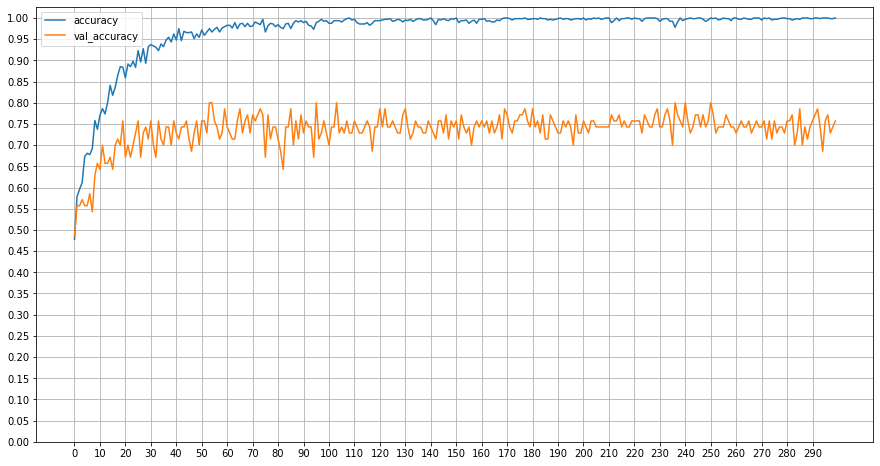
\includegraphics[scale=0.42]{image/model01.png}
  \caption{Learning curve of model 01 over 300 epochs}
\end{figure}
%% As can be seen there was a considerable gap in between the accuracy achieved on
%% the training set and the one achieved on the validation set. This meant that the
%% model was overffiting the training data and was not properly able to generalize
%% to data that it had not previously seen. For this we employed regularization.
Comme on peut le constater, il y avait un écart considérable entre la précision
obtenue sur l'ensemble d'apprentissage et celle obtenue sur l'ensemble de
validation. Cela signifie que le modèle sur-exploitait les données
d'apprentissage et n'était pas en mesure de généraliser à des données qu'il
n'avait pas vues auparavant. Pour cela, nous avons utilisé la régularisation.
\section{Regularization}
%% Regularization is a term used to designate multiple methods used to combat
%% overffiting. An overfitting model is one that is memorizing the training data
%% instead of generalizing it in order to be able to perform the same task on data
%% that it has not seen. Overfitting often happens when the model is too complex
%% for the given task (one that has too many trainable parameters). Regularization
%% involves either simplifying the model by changing its architecture or
%% constraining it in one way or another to reduce the likelihood of it memorizing
%% the training data.\\ In our case, having employed transfer learning, there was
%% a major downside in removing layers of the VGG16 model is it would mean that the
%% pretrained parameters it had learning for the imagenet task would be lost. So
%% we opted for the method of constraining the model during the learning phase. The
%% particular method that we used is called Dropout. The mehtod of Dropout involves
%% disabling learning for a random portion of the network at epoch during training.
%% This makes it difficult for the network to memorise certain aspects of the
%% training data by forcing to "look at the entire picture" of sorts. After adding
%% a regularization layer we were able to achieve an average validation accuracy of
%% 87\%.
La régularisation est un terme utilisé pour désigner plusieurs méthodes
utilisées pour lutter contre l'overfiting. Un modèle surajusté est un modèle qui
mémorise les données d'apprentissage au lieu de les généraliser afin de pouvoir
effectuer la même tâche sur des données qu'il n'a pas vues. L'overfitting se
produit souvent lorsque le modèle est trop complexe pour la tâche donnée (un
modèle qui a trop de paramètres entraînables). La régularisation implique soit
de simplifier le modèle en modifiant son architecture, soit de le contraindre
d'une manière ou d'une autre afin de réduire la probabilité qu'il mémorise les
données d'apprentissage.\\ Dans notre cas, ayant utilisé l'apprentissage par
transfert, la suppression de couches du modèle VGG16 présentait un inconvénient
majeur : cela signifiait que les paramètres pré-entraînés qu'il avait appris
pour la tâche imagenet seraient perdus. Nous avons donc opté pour la méthode
consistant à contraindre le modèle pendant la phase d'apprentissage. La méthode
particulière que nous avons utilisée est appelée Dropout. La méthode de Dropout
consiste à désactiver l'apprentissage pour une partie aléatoire du réseau à
chaque époque de la formation. Cela rend difficile pour le réseau de mémoriser
certains aspects des données d'apprentissage en le forçant à "regarder l'image
entière" en quelque sorte. Après avoir ajouté une couche de régularisation, nous
avons pu obtenir une précision de validation moyenne de 87\%.
\begin{figure}[H]
  \centering
  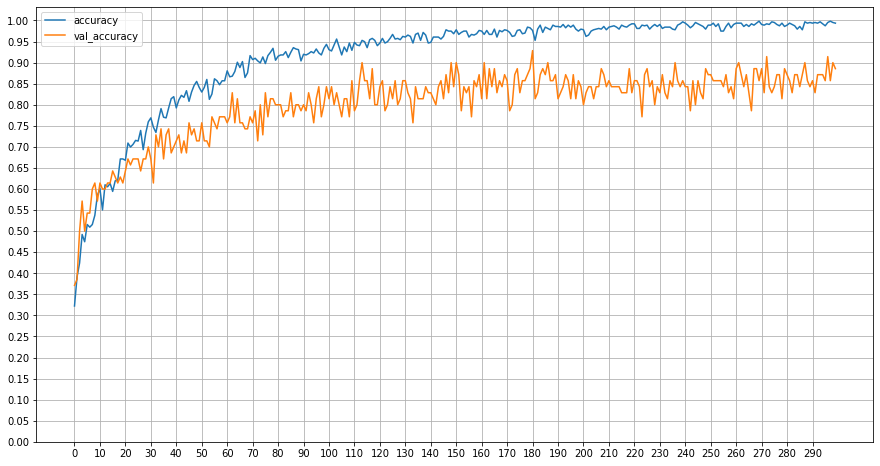
\includegraphics[scale=0.42]{image/model02.png}
  \caption{Learning curve of model 01 over 300 epochs}
\end{figure}
\section{Complete Dataset}
%% Up until now we had been working on a subset of the complete dataset. After
%% gaining access to the complete one and training our model on it. We discovered
%% that accuracy lowered significantly. Upon further invetigation we noticed that
%% the dataset that the type of images had considerably changed. Overall we have
%% discovered four types of images.
Jusqu'à présent, nous avions travaillé sur un sous-ensemble du jeu de données
. Après avoir eu accès au jeu de données complet et avoir entraîné notre modèle
sur celui-ci. Nous avons découvert que la précission a diminué de manière
significative. En poursuivant notre investigation, nous avons remarqué que le
type d'images du jeu de données avait considérablement changé. Dans l'ensemble,
nous avons découvert quatre types d'images.
\begin{figure}[H]
  \centering
  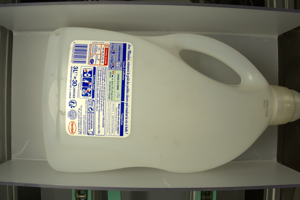
\includegraphics[scale=0.38]{image/top-dim.png}
  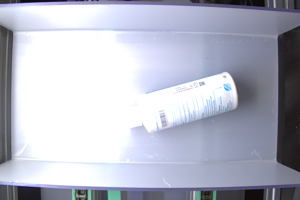
\includegraphics[scale=0.38]{image/top-lit.png}
  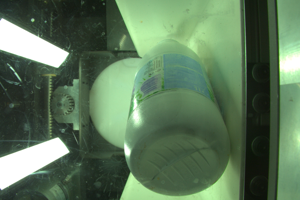
\includegraphics[scale=0.38]{image/side-vertical.png}
  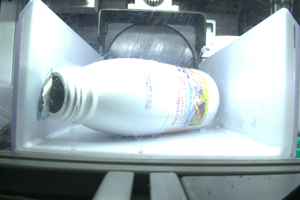
\includegraphics[scale=0.38]{image/side-horizontal.png}
  \caption{Different types of images}
\end{figure}
%% Images taken from the top and uniformaly lit, images taken from the top and with
%% higher lighting. Images taken horizontally from the side and images taken
%% vertically from the side.  Seen as takling this disparity in the data will take
%% additional work we first tested the previous VGG16 model on a subset of images
%% taken by the side and horizontally and managed to achive an average validation
%% accuracy of 89\%. And to this point we are currently testing multiple methods in
%% order to leverage as much data from the dataset as possible.
Images prises du haut et avec un éclairage uniforme, images prises du haut et
avec un éclairage plus élevé. Images prises horizontalement depuis le côté et
images prises verticalement depuis le côté. Vu que le traitement de cette
disparité dans les données nécessitera un travail supplémentaire nous avons
premièrement testé le précédent modèle VGG16 sur un sous-ensemble d'images
prises sur le côté et horizontalement et avons réussi à obtenir une précision de
validation moyenne de 89\%. Et à ce stade, nous testons actuellement plusieurs
méthodes afin d'exploiter le plus de données possible de l'ensemble de données.
\section{Final model architecture}
%% As for the time of this report this current model architecture we are using is
%% that of a modified VGG16, with four added layers. Two of these layers are Dense
%% layers, and the other two are a layer of Pooling and one of Dropout (as
%% previously detailed). The complete architecture is the following, where Conv2D
%% refers to Convolutional layers and MaxPooling2D and GlobalAveragePooling2D refer to Pooling
%% layers.
Au moment de la rédaction de ce rapport, l'architecture actuelle du modèle que
nous utilisons est celle d'un VGG16 modifié, avec quatre couches
supplémentaires. Deux de ces couches sont des couches Dense, et les deux autres
sont une couche de Pooling et une de Dropout (comme détaillé
précédemment). L'architecture complète est la suivante, où Conv2D fait référence
aux couches convolutionnelles et MaxPooling2D et GlobalAveragePooling2D font
référence aux couches de pooling.\\\\
\begin{figure}[H]
  \centering
  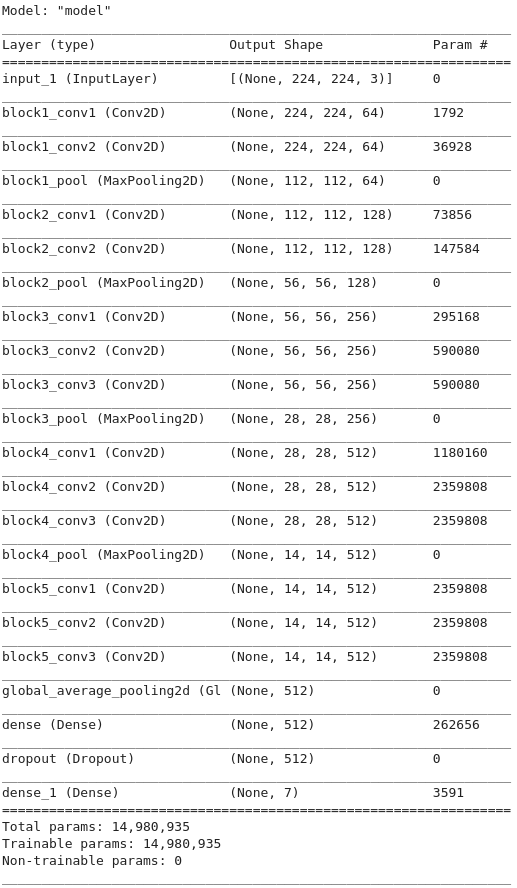
\includegraphics[scale=0.5]{image/architecture.png}
  \caption{Modified VGG16 Model}
\end{figure}
\end{document}
